\begin{landscape}
	\section{Grobkonzept}	
		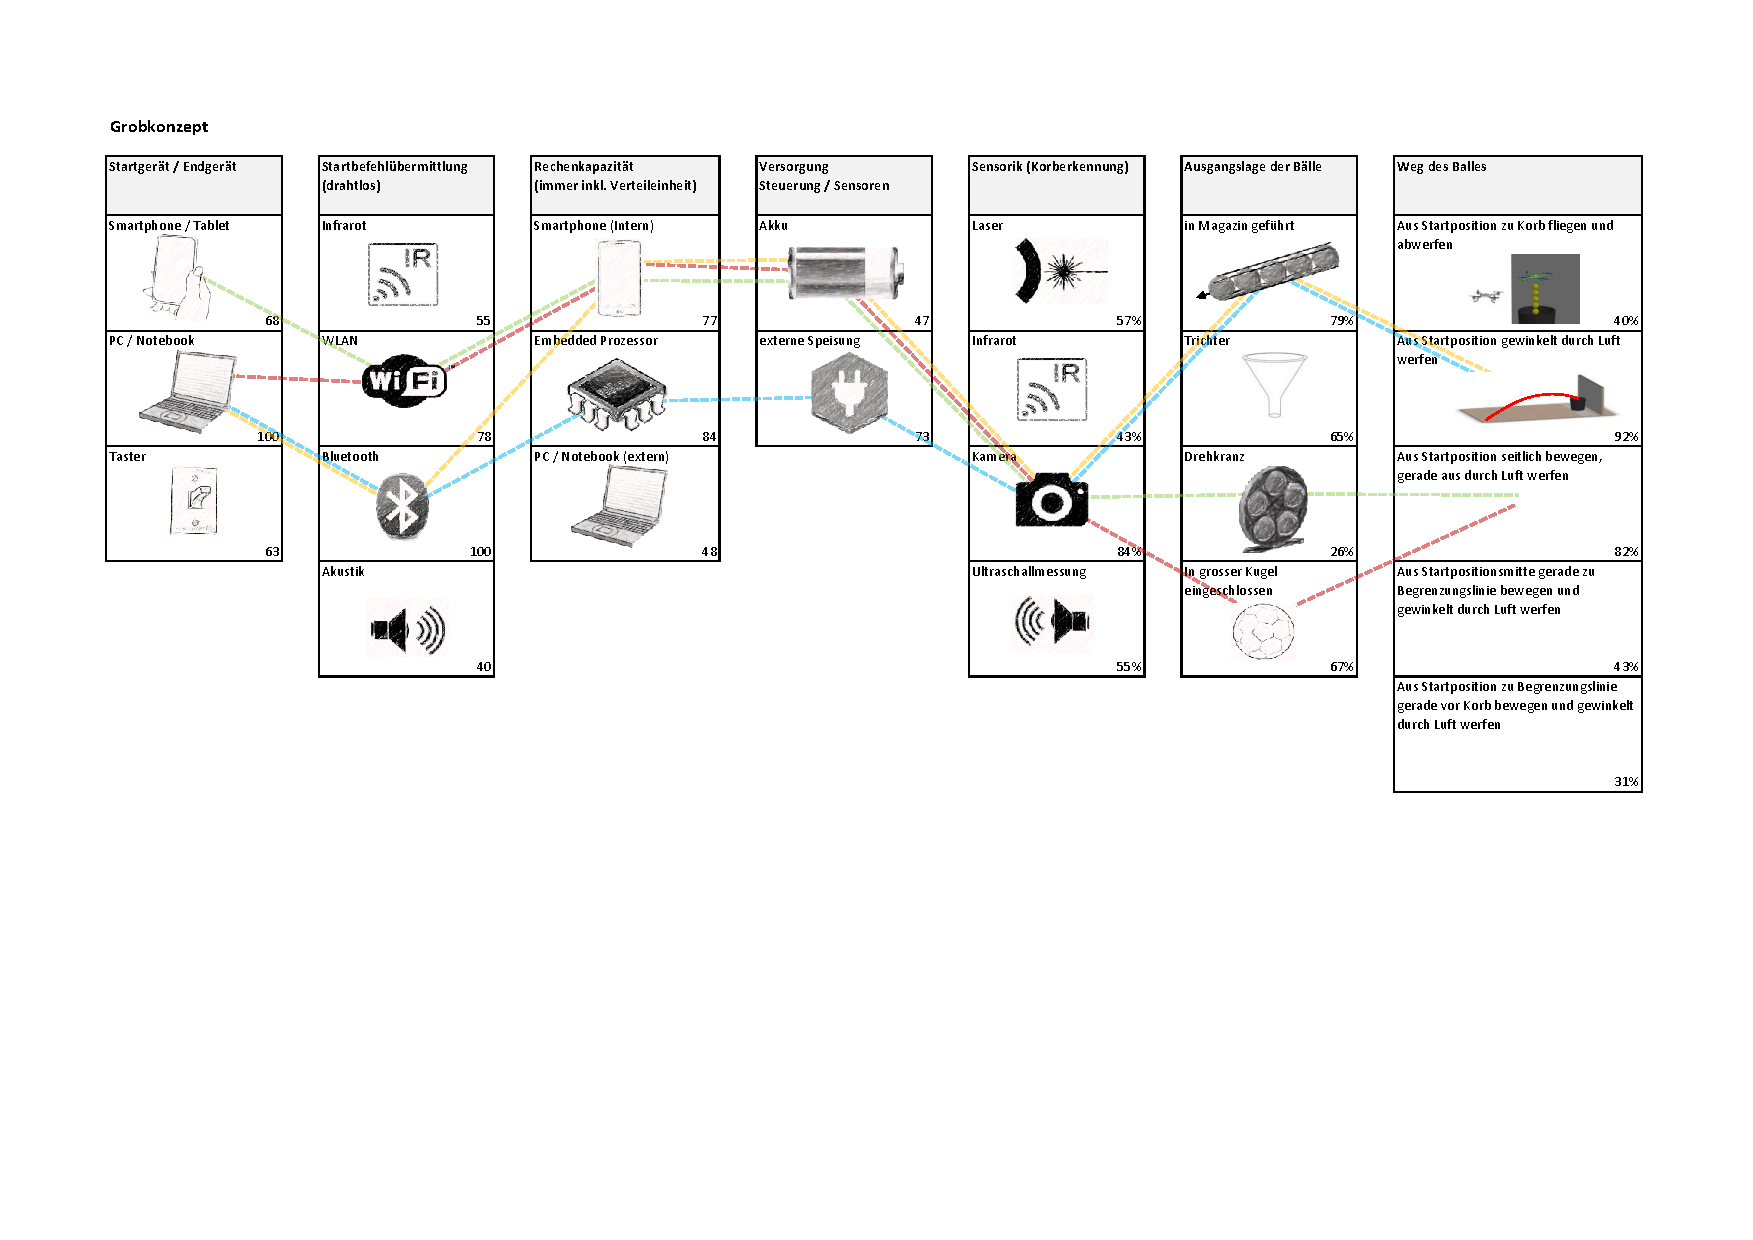
\includegraphics[page=1,scale=0.825,clip,trim=17mm 75mm 18mm 26mm]{Morphologie/Bilder/Grobkonzept.pdf}
\end{landscape} 
\textit{Die detaillierte Bewertung aller Varianten sind dem Anhang \ref{apx:BewertungGrobkonzepte} zu entnehmen.}\\
\\
Es wurden vier Varianten (orange, grün, rot, blau) gewählt. 
\begin{itemize}
	\item Blaue Variante\\
	Es wurden schlicht in jedem Teilproblem diejenige Lösung ausgewählt, welche die höchste Punktezahl in den Bewertungskriterien erreichte.
	
	\item Rote Variante\\
	Ausgangspunkt in dieser Variante ist die Auswahl, die Bälle in eine Kugel einzuschliessen. Da ein Smartphone mit integrierte Kamera verwendet wird, kann man zwei Teilprobleme mit einem Gerät lösen. Den Weg des Balles via seitliche Verschiebung wurde aufgrund der Unhandlichkeit der grossen Kugel gewählt, um den Weg kurz und einfach zu halten. Der Akku dient in dieser Variante neben der Energieversorgung auch als Ballast, um dem grossen Gewicht der Kugel entgegenzuwirken. Die Ausgabe des Startsignals mit einem Notebook und die Übertragung mit WLAN sind einfach auszuführen, beruhen auf wohlbekannten, gut dokumentierten Technologien.
	
	\item Grüne Variante\\
	Die grüne Variante wurde um die Ausgangslage der Bälle in einem Drehkranz gewählt. Den Weg des Balles via seitliche Verschiebung wurde aufgrund der Unhandlichkeit des Drehkranzes als Favorit erkoren, um den Weg kurz und einfach zu halten. Da ein Smartphone mit integrierte Kamera verwendet wird, kann man zwei Teilprobleme mit einem Gerät lösen. Der Akku dient in dieser Variante neben der Energieversorgung auch als Ballast, um dem grossen Gewicht des Drehkranzes entgegenzuwirken. Die Ausgabe des Startsignals mit einem Smartphone und die Übertragung mit WLAN sind einfach auszuführen, beruhen auf wohlbekannten, gut dokumentierten Technologien.
	
	\item Orange Variante\\
	Aus der Startposition gewinkelt werfen, ist der Ursprung der orangen Variante. Eine geführte Ausgabe aus einem Magazin hat den Vorteil, dass es mit leichten Materialen gebaut werden kann, verschiedene Formen, Winkel und Ausgabegeschwindigkeiten zur Verfügung stehen. Da ein Smartphone mit integrierte Kamera verwendet wird, kann man zwei Teilprobleme mit einem Gerät lösen. Der Akku dient in dieser Variante neben der Energieversorgung auch als Ballast und hat den schönen Nebeneffekt, dass das System Energieautark ist. Die Ausgabe des Startsignals mit einem Notebook und die Übertragung mit Bluetooth sind einfach auszuführen, beruhen auf wohlbekannten, gut dokumentierten Technologien.
	
	
\end{itemize}

\subsection{Entscheidung}
Die orange Variante bietet als gesamtes Konzept die erfolgversprechendste Lösung, bezüglich der vordefinierten Ziele der Team-Charta. Den Ball von der Startposition aus gewinkelt durch die Luft zu werfen erfordert keine zusätzlichen Bauteile um das Produkt am Boden zu verschieben. Dies minimiert einerseits den Aufwand und verringert die Fehleranfälligkeit erheblich. Die Bälle in der Ausgangslage in einem Magazin zu führen, hat den Vorteil, dass eine allfällige stückweise Ausgabe der Bälle mit wenig Aufwand hinzugefügt werden kann. Ein Smartphone mit integrierter Kamera löst die zwei Teilprobleme der Korberkennung und Rechenkapazität mit einem Gerät. Der Akku dient in dieser Variante neben der Energieversorgung auch als Ballast und hat den schönen Nebeneffekt, dass das System Energieautark ist. Die Ausgabe des Startsignals und Endsignals mit einem Notebook und die Übermittlung mit Bluetooth sind einfach auszuführen, beruhen auf wohlbekannten, gut dokumentierten Technologien.